\chapter{Introduction}

\section{Citations}
Example of text with citation \citep{Einstein}. According to \cite{latexcompanion}, this is an in-text citation. 

Table~\ref{tab:results} 

Figure~\ref{fig:giraffe}

Equation~\ref{eq:1}

\section{Math}

\[
E = mc^2
\]
\begin{equation}
E = mc^2
\label{eq:1}
\end{equation}
In line: $E = mc^2$.

\subsection{Computer code}
In line: \texttt{C++}

\begin{verbatim}
#include <stdio.h>
int main()
{
    int i, j, rows;

    printf("Enter number of rows: ");
    scanf("%d",&rows);

    for(i=1; i<=rows; ++i)
    {
        for(j=1; j<=i; ++j)
        {
            printf("* ");
        }
        printf("\n");
    }
    return 0;
}
\end{verbatim}


\begin{table}
	\centering
  \caption{Sample table of results}
  \label{tab:results}
		\begin{tabular}{lr}
      \toprule
      \textbf{Description} & \textbf{Value} \\
      \midrule
      Item 1 & $45.1$ \\
      Item 2 & $1.2$ \\
      \bottomrule
		\end{tabular}
\end{table}

\begin{figure}
	\centering
		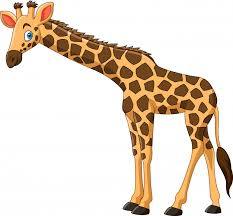
\includegraphics{images/giraffe.jpg}
	\caption{Giraffe}
	\label{fig:giraffe}
\end{figure}

